\chapter{Discussion}

\textit{``\textendash\ Those dying generations \textendash\ at their song,\\
The salmon-falls, the mackerel-crowded seas,\\
Fish, flesh, or fowl, commend all summer long\\
Whatever is begotten, born, and dies''.\\
\textemdash\ ``Sailing to Byzantium'' by William Butler Yeats }

\vspace{.2cm}

\section{Entitlements and Population}

Through the visualisation of coefficients of regular and smooth term, the positive or negative relationship between variables is clearly showed. The first step is to review the hypothesis which are made before and to see the significance.

\begin{figure}[h]
    \centering
    \caption{GAM Coefficients Summary}
    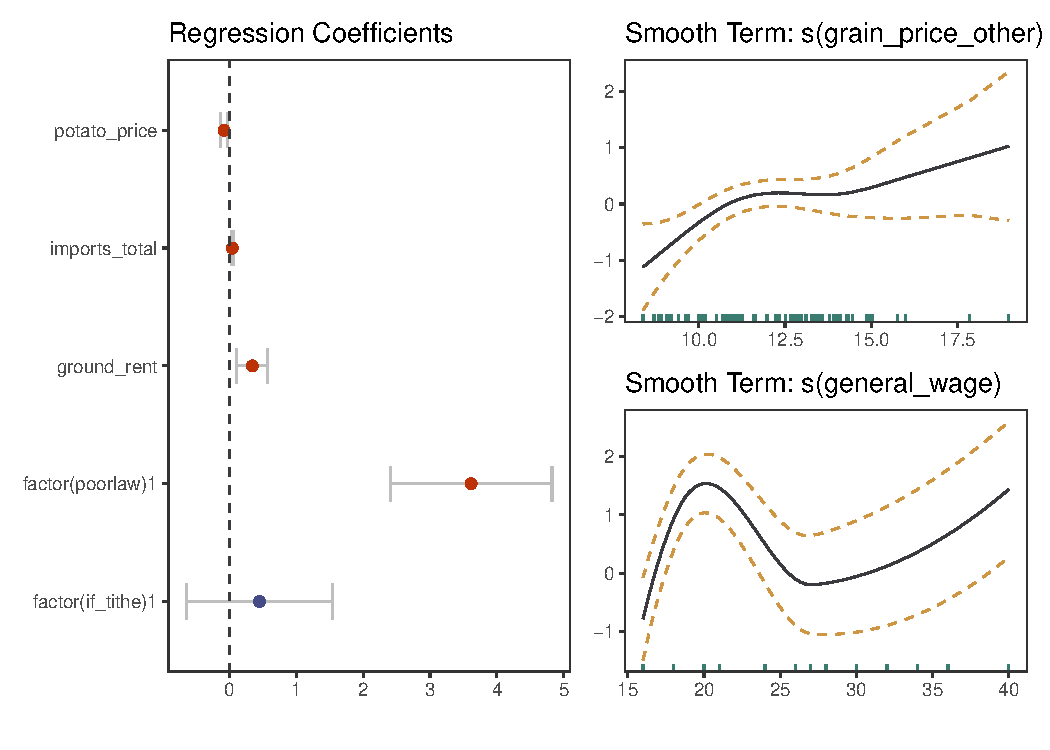
\includegraphics[width=.95\textwidth]{../03_outputs/coef.visual.pdf}
\end{figure}
\vspace{-7pt}

$H1$ describes a status between trade-based entitlement and population change, which can be proved with the coefficient of potato price but not with the smooth term trend of other grain price. This result responds to the main crop of the famine, which is the potato. As discussed earlier, the fluctuation in the price of potatoes, the most important food for livelihoods, points directly to changes in population, i.e., when the price rises, there is a significant decrease in population. However, there is a lack of consideration that the price could have a natural change with the times. Currency reforms, structure of production shifts, demographic or dominant cultural changes may directly lead to price anomalies. Anything, when related to currency and time series, should be drew conclusions carefully. Thus, $H1$ only can be partly proved with the data of potato price, that is, \textbf{A damage in people's trade-based entitlement, especially when the entitlements to get the most dominant food in diet structure is hurt, will lead to a decrease in population in a year.} As for other grain, acting as substitute products, the raise of their prices may not related to a damage in people's trade-based entitlements, or effect population less compared with the dominant food.

In fact, variables directly related to currency can be discussed together, which are other grain price, general wage and ground rent. In Ireland, price goes high because of multiple positive or negative reasons, including relationship between peasant and landlord, UK market or urbanization \citep{kennedy2014markets}. However, the significance positive coefficient of the ground rent, plus a non-significant coefficient in tithe, anyway, suggest our $H2$ is fail to prove, that is, \textbf{We do not find enough evidence to prove the casual relationship between production-based entitlement and population change.} One possible reason for this is the gap between country and urban of Ireland, more specifically, when we discuss the famine and the construction of the entitlement approach, we are in fact looking primarily at the countryside, whereas the variable of ground rent, especially when we use currency as the scale, is likely to be more associated with urban dwellers. With the rapidly urbanization of Ireland in the 19th century \citep{graham1992landlords}, it is quite possible that an increase in land rent was instead positively associated with an increase in people's entitlements.

Following the logic, the $H3$, which focus on wage is a good example to interpret. The smooth term of wage is divided into three sections obviously, and it follows the logic we use previously totally. In the first section, the raise of the wage shows a huge effect on population increase, which prove the $H3$ perfectly, while the second section suggest  the interference from inflationary or other factors, with the increase of wage population decrease, and finally, a positive relationship can be observed again. Due to we confirm the existence of interference factors, $H3$ can be proved totally, that is, \textbf{A damage in people's own-labour entitlement, or the decrease of wage, will lead to a decrease of population.} In addition, when considering the distinguish of the groups, classes or times, the difference in curvature of the curve at low and high wages is also worth to analysis. Literature shows that there is a diminishing marginal effect of wages \citep{li2012capital}, i.e. for peasants with lower wages, or in the early part of the nineteenth century, the population increase from a small wage gain was huge, whereas for the rest of the population with higher wages, or in the later part of the nineteenth century, when wages were generally higher, the stimulus of a wage increase to the population would have been much smaller.

Lastly is the Poor Law represented by $H4$, which also presents the largest positive coefficient within the key variables. 

\newpage

\section{Limitation}




